\documentclass[graybox]{svmult}

\usepackage{booktabs}
\usepackage{cite}
\usepackage[bottom]{footmisc}
\usepackage[utf8]{inputenc}
\usepackage{graphicx}
% epstopdf needs to be included after graphicx.
\usepackage{epstopdf}
\usepackage{listings}
\usepackage{makeidx}
\usepackage{multicol}
\usepackage{newtxtext}
\usepackage{newtxmath}
\usepackage{url}
\RequirePackage[l2tabu, orthodox]{nag}

% Allow PDF 1.7 documents to be included with \includegraphics
\pdfminorversion=7

\graphicspath{{./img/}}

% listing
\lstset{%
  language={C},
  basicstyle={\small\ttfamily},%
  identifierstyle={\small\ttfamily},%
  commentstyle={\small\itshape},%
  keywordstyle={\small\bfseries},%
  ndkeywordstyle={\small\ttfamily},%
  stringstyle={\small\ttfamily},%
  frame={tb},%
  breaklines=true,%
  columns=[l]{fullflexible},%
  numbers=left,%
  numberstyle={\scriptsize},%
  stepnumber=1,%
  numbersep=1em,%
  lineskip=-0.5ex,%
  mathescape,%
  xleftmargin=2em,%
  framexleftmargin=1.5em,%
}

\makeindex

\begin{document}

\title*{An MPI Framework for HPC Clusters Deployed with Software-Defined
Networking}
% Use \titlerunning{Short Title} for an abbreviated version of
% your contribution title if the original one is too long
\author{Keichi Takahashi, Susumu Date, Yasuhiro Watashiba, Yoshiyuki Kido,
Shinji Shimojo}
% Use \authorrunning{Short Title} for an abbreviated version of
% your contribution title if the original one is too long
\institute{Keichi Takahashi \at Nara Institute of Science and Technology,
8916-5 Takayama, Ikoma, Nara, Japan\\ \email{keichi@is.naist.jp}
\and Susumu Date, Yasuhiro Watashiba, Yoshiyuki Kido, Shinji Shimojo \at
Cybermedia Center, Osaka University, 5-1 Mihogaoka, Ibaraki, Osaka, Japan\\
\email{{date, watashiba-y, kido, shimojo}@cmc.osaka-u.ac.jp}}
\maketitle

\abstract*{%
SDN-enhanced MPI is a framework that integrates the network programmability of
Software-Defined Networking (SDN) with Message Passing Interface (MPI). The
aim of SDN-enhanced MPI is to improve MPI communication performance by
dynamically steering the traffic in the interconnect based on the
communication pattern of applications. A limitation in the current
implementation SDN-enhanced MPI is that multiple jobs cannot be executed
concurrently. This paper lifts this limitation  by integrating SDN-enhanced
MPI with the job scheduler. Specifically, we develop a plugin for the
scheduler to collect and transmit job information to the  interconnect
controller. A preliminary evaluation demonstrated that applications can gain
up to 2.56$\times$ speedup in communication.
}

\abstract{%
SDN-enhanced MPI is a framework that integrates the network programmability of
Software-Defined Networking (SDN) with Message Passing Interface (MPI). The
aim of SDN-enhanced MPI is to improve MPI communication performance by
dynamically steering the traffic in the interconnect based on the
communication pattern of applications. A limitation in the current
implementation SDN-enhanced MPI is that multiple jobs cannot be executed
concurrently. This paper lifts this limitation  by integrating SDN-enhanced
MPI with the job scheduler. Specifically, we develop a plugin for the
scheduler to collect and transmit job information to the  interconnect
controller. A preliminary evaluation demonstrated that applications can gain
up to 2.56$\times$ speedup in communication.
}

\section{Introduction}\label{kt:sec:i}

The demand for computing performance of high-performance computing (HPC)
clusters has been every-growing. In fact, exascale machines are now on the
horizon. To meet the sustained growth of HPC clusters, the high-performance
network that interconnects the compute nodes composing a cluster, or
\textit{interconnect}, needs to be enhanced to achieve larger scale, higher
bandwidth and lower latency. As a result, the interconnect now accounts for a
significant portion of total financial cost and power consumption of an HPC
cluster~\cite{Michelogiannakis2017}.

Until today, the established strategy for designing an interconnect has been
\textit{over-provisioning}, where extra bandwidth and routes are provisioned
in the interconnect. The reason for adopting this design strategy is two-fold.
First, networking hardware used in conventional interconnects do not allow
administrators to change their configurations on-the-fly. Therefore, the
interconnect needs to be provisioned with abundant bandwidth and routes so
that any application with arbitrary communication pattern can experience the
same degree of communication performance. Second, a production HPC cluster is
usually shared among many users where each user runs different applications.
Therefore, tailoring an interconnect to a single application with a specific
communication pattern is unrealistic.

However, an over-subscribed design is becoming increasingly challenging to
implement due to its rapidly rising financial cost and power consumption.
Meanwhile, the assumption that interconnects are static and cannot be
reconfigured does not hold anymore with the recent emergence of networking
technologies that introduces network programmability. A prominent example of
such networking technology is Software-Defined Networking~(SDN), which is a
novel networking architecture that allows administrators to dynamically and
flexibly control the network like a software. We believe that dynamically
controlling the traffic in the interconnect based on the communication pattern
of an application can alleviate traffic congestion in the interconnect and
remove the need for excessive over-provisioning.

Based on this idea, we have been developing on \textit{SDN-enhanced MPI}, a
framework that integrates Software-Defined Networking (SDN) into Message
Passing Interface~(MPI)~\cite{MPIForum2012}. The goal of this framework is to
mitigate congestion in the interconnect and improve MPI communication
performance by dynamically steering the traffic in the interconnect based on
the communication pattern of application. To this end, we have demonstrated
that individual MPI collectives are accelerated by utilizing
SDN~\cite{Dashdavaa2014,Takahashi2014}. Furthermore, we have designed and
implemented a mechanism to synchronize the progress of an application and the
reconfiguration of the interconnect~\cite{Takahashi2015,Takahashi2018}.
Furthermore, we have developed a toolset for facilitating the development of
SDN-enhanced MPI that consists of a profiler to extract communication pattern
from applications and an interconnect simulator to predict the traffic
generated in an interconnect~\cite{Takahashi2017}.

Although our work so far has successfully demonstrated that MPI applications
can be accelerated through the application of SDN, a key limitation has
remained towards the deployment of our framework on production clusters: our
current SDN-enhanced MPI framework does not support the concurrent execution
of multiple applications on a cluster. As mentioned earlier, clusters are
usually shared by many users. Therefore, the ability of running multiple jobs
on a cluster is vital for the practical use of our framework.

In this paper, we aim to lift this limitation and enhance SDN-enhanced MPI so
that multiple jobs can be executed concurrently. Specifically, we achieve this
by integrating our framework into the job scheduler of a cluster. The rest of
this paper is organized as follows. Section~\ref{kt:sec:ii} gives an overview
of the key technologies behind our proposal and clarifies the challenges to be
tackled. Section~\ref{kt:sec:iii} presents the architecture of the proposed
framework. Section~\ref{kt:sec:iv} shows the preliminary evaluation result of
the proposed framework. Section~\ref{kt:sec:v} concludes this paper and
discusses future work.

\section{Background}\label{kt:sec:ii}

\subsection{Software-Defined Networking (SDN)}

Software-Defined Networking (SDN)~\cite{Jamalian2015} is a novel networking
architecture that brings programmability into the network and allows users to
dynamically and flexibly control the network as if the network was a software.
In conventional networking architectures, the \textit{control plane}, which
makes the decision on how to handle packets, and the \textit {data plane},
which forwards packets, are tightly coupled together on a single networking
device such as a switch. In contrast, SDN separates these the two planes into
different hardware: the data plane is handled by each networking device,
whereas the control plane is handled by a centralized software controller.
Administrators are able to dynamically and flexibly control the network by
developing a controller that implements their desired network control policy.

The current de facto standard implementation of SDN is
OpenFlow~\cite{McKeown2008}. In an OpenFlow network, the data plane is handled
by OpenFlow switches, and the control plane is handled by an OpenFlow
controller. Each OpenFlow switch holds a flow table, a collection of flow
entries. A flow entry defines what action to perform on what type of packets.
The OpenFlow controller controls the traffic in the network by installing and
updating the flow table on each switch in the network. This paper assumes that
the interconnect of the cluster is built using OpenFlow switches.

\subsection{Job Scheduler}\label{kt:sec:ii-jms}

As mentioned in Sect.~\ref{kt:sec:i}, a production HPC cluster is a shared
environment. Therefore, the computing resources within the cluster need to be
efficiently managed and fairly distributed among multiple users.

To achieve this goal, the administrator of a cluster usually deploys a
\textit{job scheduler}. A job scheduler is a system that manages the computing
resources such as CPU, GPU and memory in a cluster. The job scheduler accepts
\textit{job} submissions from users, which is a request to run an application
on the cluster and a set of resource to run the application. The job scheduler
allocates computing resource in the cluster and launch the application on the
allocated computing resources. If there are insufficient available resource in
the cluster, the job will be queued for later execution. Job schedulers used
in production HPC clusters include Slurm~\cite{Yoo2003}, PBS
Professional\footnote{\url{https://www.pbspro.org/}},
Torque\footnote{\url{https://www.adaptivecomputing.com/products/torque/}} and
Grid Engine\footnote{\url{http://www.univa.com/products/}}. In this paper,
Slurm is assumed to be deployed on the cluster since it is one of the most
widely adopted free and open-source job schedulers.

\begin{figure}
    \centering
    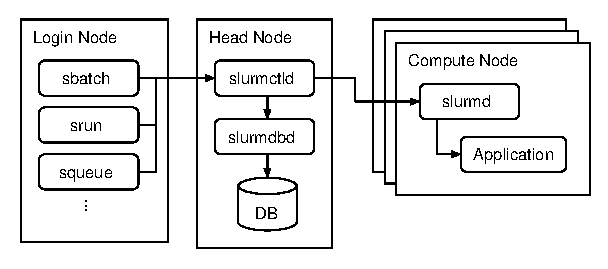
\includegraphics{slurm}
    \caption{Architecture of Slurm}%
    \label{kt:fig:slurm}
\end{figure}

Figure~\ref{kt:fig:slurm} illustrates the architecture of Slurm. Slurm employs
a \textit{master-worker} architecture like many other job schedulers. The
master, slurmctld, oversees the status of every compute node in the cluster.
It receives job submissions from users, allocates computing resources to a job
and launches the job by instructing to the workers. Optionally, slurmdbd is
used for logging and accounting purposes. Each compute node runs a worker,
slurmd, that monitors the status of the compute node, communicates with
slurmctld and launches user applications when requested by slurmctld. Users
interact with slurmctld through utilities such as sbatch (submits a job), srun
(submits an interactive job) and squeue (list queued jobs).

\subsection{Challenges}

Even though a job scheduler is useful for both administrators and users of a
cluster, it causes a major challenge in SDN-enhanced MPI\@. The interconnect
controller needs to know several information about a job to compute and
install a routing to the interconnect. This information includes:

\begin{itemize}
    \item When a job starts and finishes
    \item Which compute nodes are assigned to a job
    \item How MPI processes are distributed across the allocated compute nodes
\end{itemize}

However, this job information is only known to the job scheduler and user
application. Therefore, the job information needs to be obtained from the job
scheduler or user application and then conveyed to the interconnect manager.
In addition, the mechanism should be transparent from the users so that they
do not need to invoke a special program from their application or link a
library to their application.

\section{Proposal}\label{kt:sec:iii}

This section first briefly reviews the overall architecture of the proposed
framework. Subsequently, individual components of the framework are described
in detail.

\subsection{Overview}

The basic idea behind the proposed framework is to integrate the interconnect
manager with the job scheduler so that the reconfiguration of the interconnect
can be performed in accordance with the execution of jobs.
Figure~\ref{kt:fig:architecture} illustrates the overall architecture of the
proposed SDN-enhanced MPI framework. The proposed framework mainly consists of
three components: (1)~interconnect manager, (2)~scheduler plugin, and
(3)~OpenFlow controller. The interconnect manager is responsible for computing
optimized routes  for each job. The scheduler plugin is responsible for
collecting and submitting the job information to the interconnect manager when
a job has started or finished. The OpenFlow controller is responsible for
communicating with the OpenFlow switches and installing the routing generated
by the interconnect manager. We reuse a generic OpenFlow controller provided
by the Ryu\footnote{\url{https://osrg.github.io/ryu/}} OpenFlow framework that
provides a REST API to install, query, update and remove flows.

\begin{figure}
    \centering
    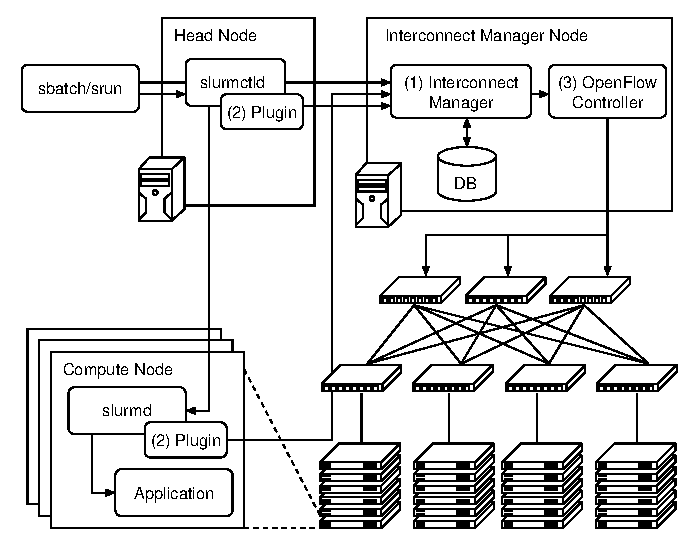
\includegraphics{architecture}
    \caption{Overall architecture of the proposed framework}%
    \label{kt:fig:architecture}
\end{figure}

The scheduler plugin and the interconnect manager communicate with
one another using RPCs. Specifically, gRPC\footnote{\url{https://grpc.io/}}, which is an
RPC framework built on top of HTTP/2, is used. The main reason behind this
design choice is because gRPC can automatically generate server and client
codes from an interface definition of remote procedures. Therefore, using gRPC
saves much development effort than implementing our own protocol upon raw
TCP/IP\@.

\subsection{Scheduler Plugin}

The scheduler plugin is responsible for collecting and sending information
about a job every time a job has started or finished. As described earlier,
the scheduler decides when to run each job. Furthermore, the node allocation
and process mapping are unknown until the job starts. Therefore, a mechanism
is needed to notify the interconnect manager about this information.

For this reason, we utilize a builtin plugin mechanism of Slurm, which is
called Slurm Plug-in Architecture for Node and job Control (SPANK). SPANK
allows developers to easily customize the job startup and cleanup routines of
Slurm. SPANK plugins are not linked with Slurm itself and can be loaded during
runtime. In addition, SPANK allows developers to add new options to the job
script and job submission commands.

Our SPANK-based plugin is loaded by all Slurm components and performs the
following operations:

\begin{itemize}
    \item \textbf{sbatch/srun}: When a job is submitted by a user via sbatch
        or srun, our plugin sends the ID and name of the job, uid of the
        submitter, number of processes and communication pattern of the
        application to the interconnect manager. Currently the user
        needs to manually specify the communication pattern in the job script
        as shown in Listing~\ref{kt:lst:script}.
    \item \textbf{slurmd}: When slurmd is about to launch a job on a compute
        node, our plugin sends the ID and name of the job, compute node ID,
        and MPI rank number to the interconnect manager. This is used by the
        interconnect manager to obtain the node allocation and process
        mapping. After this information is sent over to the interconnect
        manager, the plugin blocks until the routing are computed and
        installed to the interconnect. Once the routing is setup, the plugin
        returns control to Slurm. After that, the user application starts.

        When a job has finished, the same information is send over to the
        interconnect manager and blocks until the routings are uninstalled
        from the interconnect. After that, the rest of the cleanup is
        completed.
\end{itemize}

\begin{lstlisting}[float,caption=An example of a job script,label=kt:lst:script]
#!/bin/bash
#
#SBATCH --job-name=cg-benchmark
#SBATCH --ntasks=128
#SBATCH --time=01:00:00
#
#SBATCH --comm-pattern=cg-c-128
\end{lstlisting}

All of the above operations are performed transparently from the user
application. In other words, the user application does not need to be modified
nor a special program needs to be invoked.

\subsection{Interconnect Manager}

The primary purpose of the interconnect manager is to compute and install
optimal routing for each job.

To compute the optimal routing for a job, the interconnect manager needs to
know how the MPI processes constituting a job is laid out on the cluster.
This information are received from the scheduler plugin integrated into the
Slurm scheduler. Furthermore, the communication pattern of a job is also
received from the plugin if the user has specified the communication pattern.
This job information is persisted on an external database (currently
SQLite\footnote{\url{https://www.sqlite.org/index.html}} is used) for
fault-tolerance.

Once the scheduler has received the job information, the manager computes the
optimal routing for the job. The actual routing algorithm itself is pluggable
and can be swapped out. The computed routing is then installed through the
OpenFlow controller to each switch in the interconnect.

\section{Evaluation}\label{kt:sec:iv}

In this section, we conduct a preliminary evaluation to assess if applications
can be accelerated using our proposed framework.

\subsection{Evaluation Environment}

The evaluation experiment was conducted on a small-scale cluster composed of
20 compute nodes connected through a two-tier fat-tree interconnect
(Fig.~\ref{kt:fig:cluster}). Each compute node is equipped with two quad-core
Intel Xeon E5520 CPUs. In total, there are 160 CPU cores in the cluster. A
single NEC PF5240 OpenFlow switch is divided into six virtual switches to
compose a fat-tree topology. D-mod-K routing~\cite{Rodriguez2009} was chosen
as the representative example of a conventional routing algorithm. D-mod-K
routing statically distributes traffic flows across multiple paths in the
interconnect based on the destination of a flow.

\begin{figure}
    \centering
    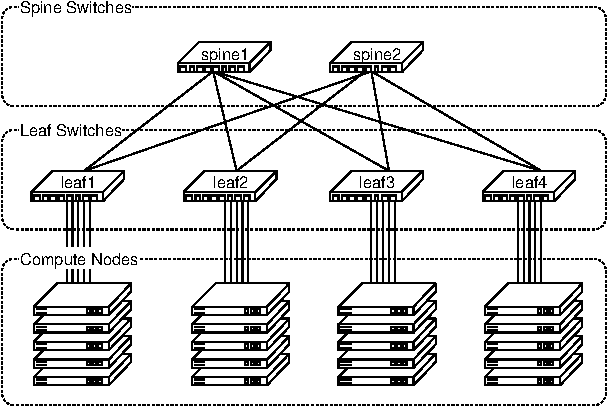
\includegraphics{evaluation_cluster}
    \caption{Cluster used for evaluation}%
    \label{kt:fig:cluster}
\end{figure}

We executed a set of benchmarks on a cluster and compared the communication
time of each benchmark with and without our framework.
Table~\ref{kt:tbl:miniapps} shows a list of communication benchmarks used in
the evaluation. CG and FT are taken from the NAS parallel benchmark
suite~\cite{Bailey1991}. Stencil2D, Stencil3D and SpMV were developed by us.
All benchmarks were executed using 160 processes. In other words, we ran a
single process for every CPU core in the cluster.

\begin{table}
\caption{Benchmarks used in the evaluation}%
\label{kt:tbl:miniapps}
\begin{tabular}{ll}
\toprule
Name      & Description \\ \midrule
CG        & Solves a sparse linear system using the Conjugate Gradient method \\
FT        & Solves partial differential equation using FFT and IFFT           \\
Stencil2D & A two-dimensional stencil solver                                  \\
Stencil3D & A three-dimensional stencil solver                                \\
Butterfly & An Allreduce kernel commonly seen in deep learning                \\
SpMV      & A sparse matrix-vector multiplication kernel                      \\ \bottomrule
\end{tabular}
\end{table}

\subsection{Evaluation Result}

Figure~\ref{kt:fig:benchmark} shows the relative speedup of MPI communication
when using our framework. CG, Butterfly, and SpMV achieved 1.29$\times$,
1.18$\times$, and 2.56$\times$ speedup, respectively. In contrast, FT,
Stencil2D, and Stencil3D did not exhibit a clear performance gain by using our
framework.

We believe that this trend can be explained from the following reasons. FT
performs all-to-all communication between processes. This complete lack of
locality makes it challenging to efficiently map the communication pattern
into the interconnect. In contrast, Stencil2D and Stencil3D perform nearest
neighbor communication in a two-dimensional or three-dimensional process grid.
As a result, most of the communication happens within a compute node or within
a leaf switch, which makes the difference in routing algorithms irrelevant.

The three benchmarks that benefited from our framework (CG, Butterfly and
SpMV) require both local and remote communication. Therefore, there is a
chance to improve the load balancing of flows by considering the communication
pattern of benchmarks.

\begin{figure}
    \centering
    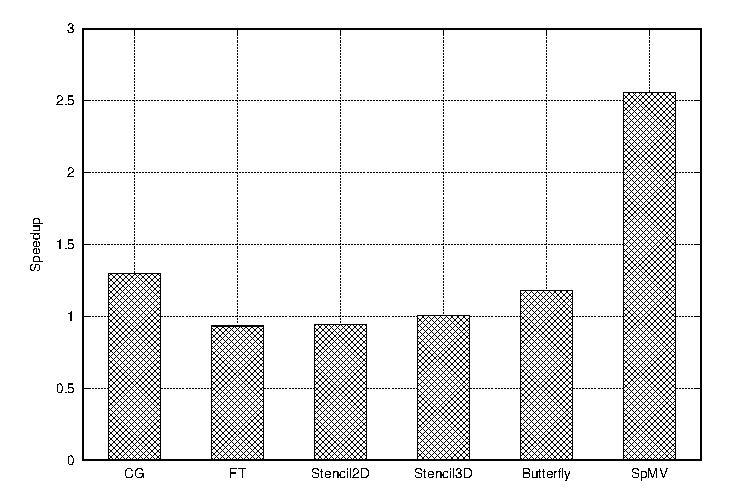
\includegraphics{benchmark_result}
    \caption{Benchmark results using miniapps}%
    \label{kt:fig:benchmark}
\end{figure}

\section{Conclusion}\label{kt:sec:v}

SDN-enhanced MPI aims to improve MPI communication performance by dynamically
steering the traffic in the interconnect based on the communication pattern of
applications. This paper tackled the limitation of SDN-enhanced MPI that
multiple jobs cannot be executed concurrently. Specifically, we integrated
SDN-enhanced MPI with the job scheduler. A preliminary evaluation conducted
using benchmarks demonstrated that our framework achieves up to 2.56$\times$
speedup in communication. As a future work, we would like to evaluate our
framework using a large job set containing diverse real-world applications.

\begin{acknowledgement}
This work was supported by JSPS KAKENHI Grant Number 17K00168.
\end{acknowledgement}

\bibliographystyle{spmpsci}
\bibliography{references}

\end{document}
